%! TEX root = ../main.tex
% ============================================================
% IMMUTABLE — generated automatically, do not edit this block
%   script          : plotter.py::plot_damping_freq
%   plot_type       : damping_freq
%   chapter         : 05
%   panel           : all, no
%   wind            : lowest, no
%   amplitude       : 0.1
%   frequency       : 1.3
%   probes          : 1, 2, 3, 4
%
% PANELS AVAILABLE:
%   FIGURES/05_damping_freq_allpanel-lowestwind-amp0100-freq1300-probe1og2og3og4.pdf
%   FIGURES/05_damping_freq_allpanel-nowind-amp0100-freq1300-probe1og2og3og4.pdf
%   FIGURES/05_damping_freq_nopanel-lowestwind-amp0100-freq1300-probe1og2og3og4.pdf
%   FIGURES/05_damping_freq_nopanel-nowind-amp0100-freq1300-probe1og2og3og4.pdf
% ============================================================
\begin{figure}[htbp]
  \centering
  \begin{subfigure}[b]{0.48\linewidth}
    \centering
    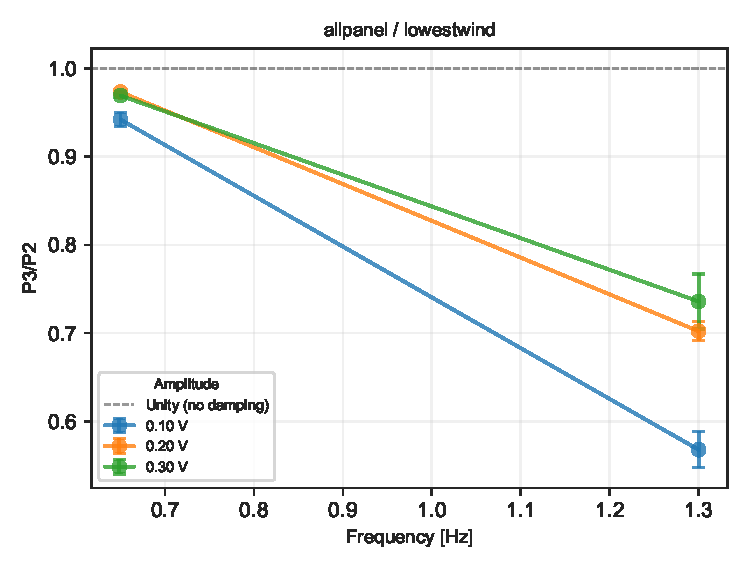
\includegraphics[width=\linewidth]{FIGURES/05_damping_freq_allpanel-lowestwind-amp0100-freq1300-probe1og2og3og4.pdf}
    \caption{TODO}
    \label{fig:TODO_1og2og3og4}
  \end{subfigure}
  \hfill
  \begin{subfigure}[b]{0.48\linewidth}
    \centering
    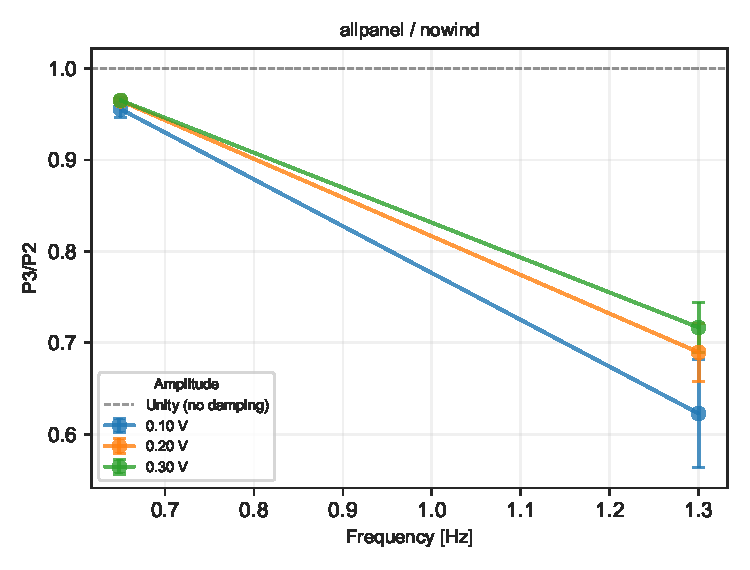
\includegraphics[width=\linewidth]{FIGURES/05_damping_freq_allpanel-nowind-amp0100-freq1300-probe1og2og3og4.pdf}
    \caption{TODO}
    \label{fig:TODO_1og2og3og4}
  \end{subfigure}
  \hfill
  \begin{subfigure}[b]{0.48\linewidth}
    \centering
    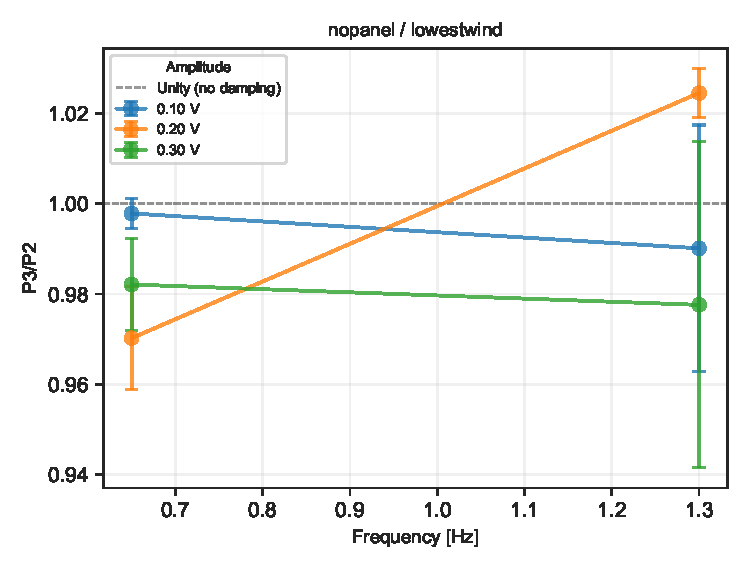
\includegraphics[width=\linewidth]{FIGURES/05_damping_freq_nopanel-lowestwind-amp0100-freq1300-probe1og2og3og4.pdf}
    \caption{TODO}
    \label{fig:TODO_1og2og3og4}
  \end{subfigure}
  \hfill
  \begin{subfigure}[b]{0.48\linewidth}
    \centering
    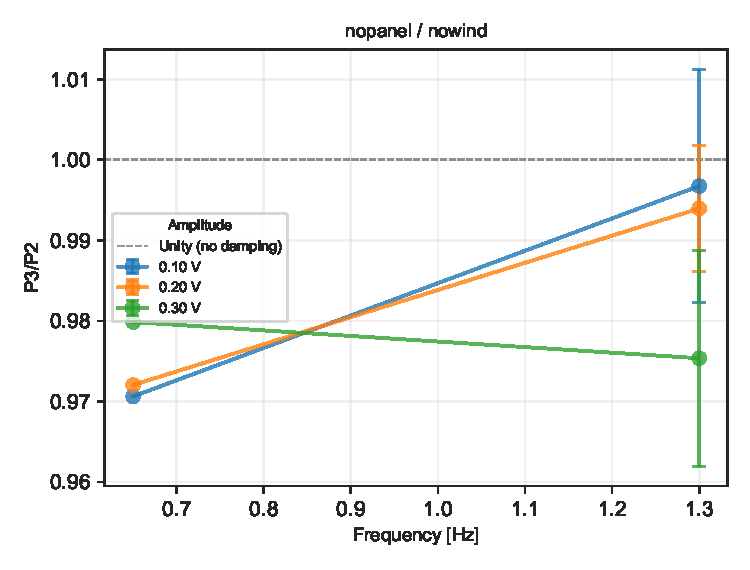
\includegraphics[width=\linewidth]{FIGURES/05_damping_freq_nopanel-nowind-amp0100-freq1300-probe1og2og3og4.pdf}
    \caption{TODO}
    \label{fig:TODO_1og2og3og4}
  \end{subfigure}
  \caption[Short caption for LOF]{
    % TODO: write caption
  }
  \label{fig:TODO_p0100-freq1300-probe1og2og3og4}
\end{figure}
